% manuale beamer http://www.ctan.org/tex-archive/macros/latex/contrib/beamer/doc/beameruserguide.pdf
% **************************************************************
% Hi! Edit this file for your presentation!
% **************************************************************

% ==================///==================///==================///
% ==================/// LATEX'S STUFF
% ==================///==================///==================///
% !TEX root = main.tex
\documentclass[aspectratio={169}]{beamer}
\usepackage{amsfonts,amsmath,oldgerm}
\usetheme{_statale}
\usefonttheme[onlymath]{serif}

\newcommand{\testcolor}[1]{\colorbox{#1}{\textcolor{#1}{test}}~\texttt{#1}}
\newcommand{\hrefcol}[2]{\textcolor{cyan}{\href{#1}{#2}}}
\titlebackground*{assets/background}

\usepackage{tikz}
\usetikzlibrary{arrows.meta, backgrounds, calc, chains, fit, graphs, graphdrawing, graphdrawing.layered, intersections, positioning, shadings, shapes, shapes.geometric, shapes.misc}

\tikzset{%
	base/.style = {
			% minimum width=1cm,
			% minimum height=1cm,
			text centered,
			% font=\sffamily,
			inner sep=0.5em,
		},
	boxes/.style = {
			base,
			draw=black,
			rectangle,
		},
	rboxes/.style = {
			boxes,
			rounded corners
		},
	arrow_label/.style = {
			base,
			midway,
			% sloped,
			fill=white, anchor=center,
			inner sep=0.25em
		}
}

% for appendix
\usepackage{appendixnumberbeamer}

% ==================///==================///==================///
% ==================/// SPLASH PAGE
% ==================///==================///==================///

\title{Design e Sviluppo di una Soluzione per la Valutazione di Sistemi Distribuiti}
\course{Laure Triennale in Sicurezza dei Sistemi e delle Reti Informatiche}
\author{\href{mailto:enea.manzi@studenti.unimi.it}{Enea Manzi}}
\IDnumber{987326}
\date{
	Relatore: Prof. Marco Anisetti\\
	Correlatore: Dottor. Filippo Berto\\
	22 Ottobre 2024}

% ==================///==================///==================///
% ==================/// START PRESENTATION
% ==================///==================///==================///

\begin{document}
\newcommand{\highlightprofilecolor}{LightGoldenRod!100}

\tikzset{
	entity/.style={
			draw,
			ellipse,
			very thin
		},
	artifact/.style={
			rectangle,
			draw,
			rounded corners,
			fill=VeryLightGrey!50
		},
	service/.style={
			chamfered rectangle,
			chamfered rectangle angle=30,
			draw,
			%fill=VeryLightGrey!120
		},
	every node/.style={
			font={\scriptsize},
			text centered,
		},
	on link/.style={
			fill=white,
		},
	connector/.style={
			>=stealth,
		},
	connector assurance/.style={
			>=Stealth,
			dashed
		},
	on slide/.code args={<#1>#2}{%
			\only<#1>{\pgfkeysalso{#2}}%
		},
	highlight base/.style={
			very thick
		},
	highlight/.style={
			highlight base,
			fill=LightGoldenRod,
		},
	highlight profile/.style={
			\highlightprofilecolor
		},
	highlight double/.style={
			double=LightGoldenRod
		},
	highlight text/.style={
			text=Goldenrod,
		},
	highlight link/.style={
			%thick,
			color=Goldenrod
		},
	highlight light/.style={
			fill=LightGoldenRod!50
		},
	highlight very light/.style={
			fill=LightGoldenRod!20
		},
	element/.style={
			inner sep=1.5pt,
			font=\footnotesize
		},
	connector/.style={
			>=Stealth,
		},
	lattice layer label/.style={
			text width=2.9cm,
			font={\footnotesize},
		},
	not chosen color/.style={
			black!50
		},
	lattice layer separator/.style={
			dashed,
		},
	service label/.style={
			fill=white,
			circle,
			draw,
			very thick,
			inner sep=2.5pt,
		},
	lattice element bound/.style={
			fill=black!15,
			double
		},
	lattice element selected/.style={
			fill=Goldenrod!15,
			double
		},
	lattice element not chosen/.style={
			not chosen color,
			densely dotted
		},
	lattice element not chosen link/.style={
			not chosen color,
			densely dotted
		},
	service element not chosen/.style={
			text=black!50,
			draw=black!50,
			dashed,
		},
	header/.style={
		},
	main box/.style={
			font={\small}
		},
	link/.style={
			>=Latex,
		},
	activity/.style={
			fill=white
		},
	% for cert history
	arrow/.style={
			draw,
			minimum height=1cm,
			inner sep=2pt,
			shape=signal,
			signal from=west,
			signal to=east,
			signal pointer angle=110,
			top color=DarkBlue,
			bottom color=DarkBlue,
			text=White,
			text width=.24\textwidth,
			font = {\small}
		},
	desc/.style={
			%text width=3.9cm,
			text width=.22\textwidth,
			fill=VeryLightGrey,
			%minimum height=1cm,
			%anchor=south
			% text depth=1cm,
			rectangle,
			font = {\footnotesize}
		},
	link comment/.style={
			dashed
		}
}

\maketitle

\footlinecolor{maincolor}

% ==================///==================///==================///
% ==================/// BODY'S PRESENTATION
% ==================///==================///==================///



%\begin{frame}{Table of Contents}
%	\tableofcontents
%\end{frame}
% TODO rimuovere
%\section{Contesto}

% SECONDO FILIPPO SI POSSO FORSE UNIRE PER RISPARMIARE TEMPO
\begin{frame}{Contesto}
  \begin{columns}
    \begin{column}{.7\textwidth}
      \begin{itemize}
        \item Esigenze di \alert{performance elevate}

        \item \alert{Limiti dei sistemi centralizzati}
        
        \item Avvento del \alert{cloud computing}:
        
          \begin{itemize}
            \item Sistemi \alert{decentralizzati}
            \item Sistemi \alert{distribuiti}
            \item Architetture basate su \alert{microservizi}
          \end{itemize}

      \end{itemize}
    \end{column}

    \begin{column}{.2\textwidth}
      
\includegraphics[scale=.2]{assets/icon/01contesto_distributed_system.png}
    \end{column}
  \end{columns}
  
\end{frame}


\begin{frame}{Contesto}
  \begin{columns}
    \begin{column}{.8\textwidth}
      \begin{itemize}
        \item Necessità di strumenti di \alert{monitoraggio avanzato}

        \item Raccogliere \alert{informazioni} dai \alert{diversi sistemi}

        \item Necessità di avere \alert{garanzie sui servizi}

        %L'assurance permette 

      \end{itemize}
      \textbf{Obiettivo finale}: valutare il \alert{comportamento complessivo} del sistema
    \end{column}

    \begin{column}{.2\textwidth}
      
\includegraphics[scale=.2]{assets/icon/01contesto_assurance_distributed_system.png}
    \end{column}
  \end{columns}

  
\end{frame}

% TODO rimuovere
%\section{Gaps}

%SECONDO FILIPPO è MEGLIO TENERE QUESTA AL POSTO DI QUELLA PRIMA
\begin{frame}{Gaps}
  \begin{columns}
    \begin{column}{.7\textwidth}
      \begin{itemize}%[<+->]
        \item \textbf{G1 Generalizzabilità} Necessità di un sistema di valutazione \alert{generico} che si \alert{interfacci} a vari strumenti di \alert{monitoraggio}
  
        \item \textbf{G2 Valutazioni Performance} Focus ristretto su aspetti di \alert{performance}, peccando di un'approccio \alert{olistico e continuativo} che valuti il \alert{comportamento} del sistema
  
        %detta da filippo come G3
        \item \textbf{G3 Elasticità Contratti} Framework attuali non permettono l'\alert{elasticità} che cerchiamo
        
      \end{itemize}
    \end{column}

    \begin{column}{.2\textwidth}
      %
\includegraphics[scale=.2]{assets/icon/motivazioni_icon.png}
      
\includegraphics[scale=.2]{assets/icon/02motivazioni_litterature_gaps.png}
    \end{column}
  \end{columns}
  
\end{frame}

% TODO rimuovere
%\section{Obbiettivi}

%sembra OK
\begin{frame}{Obbiettivi}
  \begin{columns}
    \begin{column}{.7\textwidth}
      \begin{itemize}%[<+->]
        \item \textbf{O1}: \alert{Estensione dell'Assurance Engine} per supportare il monitoraggio basato su \alert{Elasticsearch}
        
        \item \textbf{O2}: Implementazione di \alert{contratti} basati su \alert{\textit{evidence}} per eseguire \alert{valutazioni} di PNF 
  
        \item \textbf{O3}: Valutazione sperimentale delle \alert{performance del sistema} in un cluster Kubernetes
      \end{itemize}
    \end{column}

    \begin{column}{.2\textwidth}
      
\includegraphics[scale=.16]{assets/icon/03obbiettivi_objectives.png}
    \end{column}

  \end{columns}
  
\end{frame}


	

% TODO rimuovere
%\section{PNF + Metodologia Assurance}

\begin{frame}{Processo di Assurance e Proprietà}
  \begin{itemize}
    \item Necessità di un nuovo \alert{processo di assurance} per \alert{valutare} sistemi distribuiti su \alert{Proprietà Non Funzionali}
    
    \item \textbf{Verifiche di Assurance}: valutare se un sistema \alert{soddisfa i contratti} definiti, implicando la \alert{garanzia di \textbf{proprietà}} specifiche
    % i contratti sono soddisfatti
    % le proprietà sono garantire
    % soddisfando un requisito implica che ho una certa garanzia
    \begin{itemize}
      \item Valutazione \alert{continuativa}
      \item Valutazione \alert{su richiesta}
    \end{itemize}

    \item \textbf{Proprietà}: definiscono delle caratteristiche \alert{comportamentali} del sistema \textit{(Scalabilità, Affidabilità, Confidenzialità, Integrità, Disponibilità, ...)}

  \end{itemize}
\end{frame}


\begin{frame}{Metodologia di Assurance}
  \begin{columns}
    \begin{column}{.6\textwidth}
      \begin{itemize}%[<+->]
        \item \textbf{Metriche}: misurano gli \alert{stati} rilevanti del sistema

        \item \textbf{Evidence}: \alert{dati} raccolti dalle metriche, utilizzati come \alert{prove per i contratti} 
        
        \item \textbf{Contratti}: \alert{verificano} formalmente la validità di \alert{PNF} 

        \item \textbf{Report}: lista delle \alert{proprietà valutate} con il \alert{relativo esito} e le evidence a supporto

      \end{itemize}
      \vspace{1em}
    \end{column}

    \begin{column}{.4\textwidth}
      \centering
      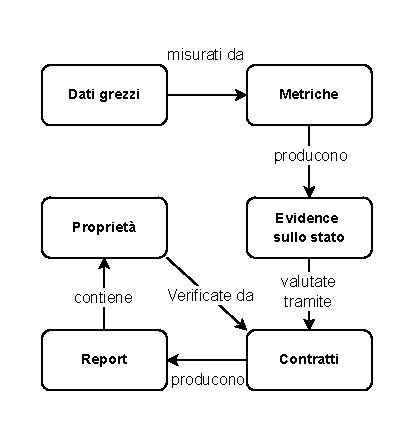
\includegraphics[width=\textwidth]{assets/metriche-contratti.drawio.pdf}
    \end{column}

  \end{columns}
\end{frame}

% TODO rimuovere
%\section{Implementazione del Sistema}


% OK DA FILIPPO
\begin{frame}{Assurance Engine ed Elasticsearch}
  \begin{itemize}


    \item L'Assurance Engine \alert{implementa} il \textbf{processo di assurance} precedente \alert{interagendo} con svariati \alert{sistemi di monitoring} (Elasticsearch,Prometheus)
    % prima erano astratti, questa è la concretizzazione
   
    \item \alert{API REST} esposte tramite OpenAPI per interagire con l'engine
    
    \item Integrazione di \alert{Elasticsearch} con l'Assurance Engine come \alert{strumento di monitoring}
    % per la raccolta, analisi e ricerca dei dati

    \begin{itemize}
      \item Efficienza nella \alert{raccolta continua} di dati, nella \alert{ricerca} e nell'\alert{analisi}
      
      %\item \alert{Scalabilità} del sistema
    \end{itemize}
  \end{itemize}
\end{frame}


\begin{frame}{Necessità e Vantaggi del Framework Intermediario}
  \begin{itemize}
    \item \alert{Estende} le capacità di Elasticsearch, utilizzando il linguaggio di programmazione \alert{Rust} 
    
    \item Infrastruttura \alert{request-reflector} 
    
    \item Fornisce \alert{scalabilità} e \alert{replicabilità senza coordinazione}:
    %L’Assurance Engine viene eseguito su un cluster Kubernetes
    
    \begin{itemize}
      \item Sistema deployato come \alert{una o più} istanze
      %\alert{Network load balancer} gestisce il traffico

      \item Istanze \alert{intercambiabili} e \alert{stateless} non necessitano di coordinazione aggiuntiva
      
      %\item Richieste gestibili da qualsiasi istanza, assicurando \alert{consistenza} e \alert{disponibilità}
    \end{itemize}
  \end{itemize}
\end{frame}


% ANCHE QUESTO SECONDO FILIPPO SI POTREBBE TAGLIARE
\begin{frame}{Funzionamento dell'Assurance Engine}

  \begin{enumerate}
    \item \alert{Richiesta} POST all'endpoint dell'Assurance Engine
    
    \item Valutazione di un contratto in \alert{tre fasi}:
    
    \begin{enumerate}
      \item \textbf{Measurement collection}: interrogazione dei \alert{servizi di monitoring} %tramite metriche
      
      \item \textbf{Contract evaluation}: valutazione dei \alert{contratti} 
      %tramite un confronto tra i parametri e le \alert{evidence} raccolte
      
      \item \textbf{Report composition}: restituzione del \alert{risultato} della valutazione %in formato JSON
    \end{enumerate}
  \end{enumerate}
\end{frame}

% TODO rimuovere
%\section{Conclusioni}


% TODO da modificare secondo chiamata filippo
% dice che bisogna dire come sono stati fatti i benchmark senza perdere tempo su risultati e anomalie
\begin{frame}{Valutazione sperimentale}
  \begin{itemize}
      \item Benchmark \alert{performance} esecuzione metriche e contratti
      
      \item Analisi in diverse circostanze
 
      \item Risultati: 
      \begin{itemize}
        \item \alert{efficienza} nella \alert{raccolta} e \alert{valutazione} di evidence tramite \textit{metriche} e \textit{contratti}
        
        \item \alert{latenza} di rete
        
        %\item \alert{minimo impatto} sulle risorse del sistema
        
        
      \end{itemize}
  \end{itemize}
\end{frame}


\begin{frame}{Conclusioni}
  \begin{columns}
    \begin{column}{.7\textwidth}
      \begin{itemize}
        \item \alert{Metodologia} innovativa di \alert{Assurance continuativa}
        
        \item Estensione \alert{ Assurance Engine} integrandolo con \alert{Elasticsearch}

        \item Implementazione di \alert{metriche e contratti formali}
        
        \item Risultati sperimentali confermano l'\alert{efficienza} del sistema
      \end{itemize}

      \vspace{1em}
      Fornisce complessivamente un sistema \alert{generico}, \alert{flessibile} e \alert{specializzabile} per verifiche di assurance
    \end{column}

    \begin{column}{.3\textwidth}
      
\includegraphics[scale=.2]{assets/icon/06conclusion_done_list.png}
    \end{column}
  \end{columns}

\end{frame}


\begin{frame}{Lavori futuri}
  \begin{columns}
    \begin{column}{.7\textwidth}
      \begin{itemize}
        \item \alert{Integrazione} con ulteriori tecnologie di monitoraggio
        \item Sviluppo di nuovi \alert{contratti} più complessi
        \item Applicazione del sistema ad \alert{ambienti in produzione} 
        %\item Valutazione della \alert{scalabilità} dell'Engine
        %usare più deployment e vedere come vanno i benchmark
      \end{itemize}
    \end{column}

    \begin{column}{.3\textwidth}
      
\includegraphics[scale=.2]{assets/icon/06conclusion_future_work.png}
    \end{column}
  \end{columns}
  
\end{frame}






% ==================///==================///==================///
% ==================/// END PRESENTATION
% ==================///==================///==================///

\backmatter

\thispagestyle{empty}
\mbox{}
\clearpage
\setcounter{page}{1}

\appendix

\begin{frame}{Assurance methodology}
  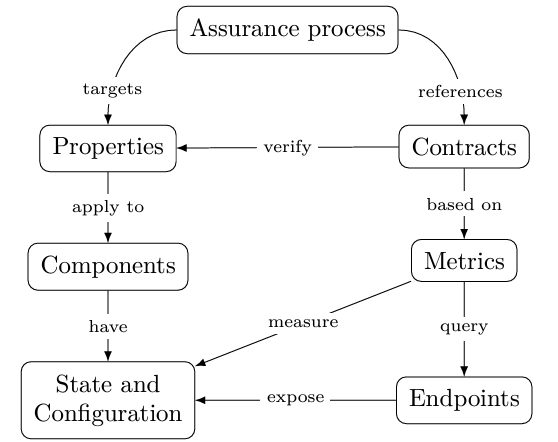
\includegraphics[width=\textwidth,height=0.9\textheight,keepaspectratio]{assets/backup_figures/01_assurance_methodology.png}
\end{frame}

\begin{frame}{Assurance process}
  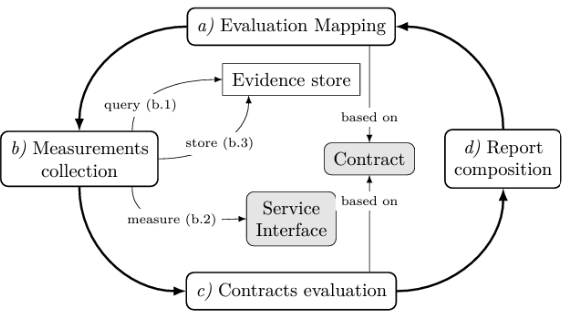
\includegraphics[width=\textwidth,height=0.9\textheight,keepaspectratio]{assets/backup_figures/02_assurance_process.png}
\end{frame}

\begin{frame}{Certification process}
  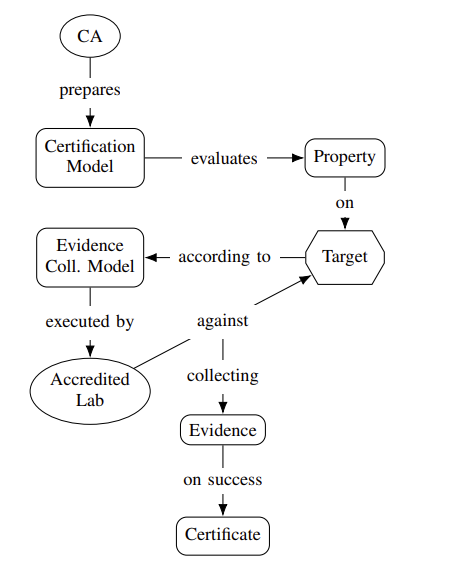
\includegraphics[width=\textwidth,height=0.98\textheight,keepaspectratio]{assets/backup_figures/03_certification_process.png}
\end{frame}

\begin{frame}{Diagramma funzionamento}
  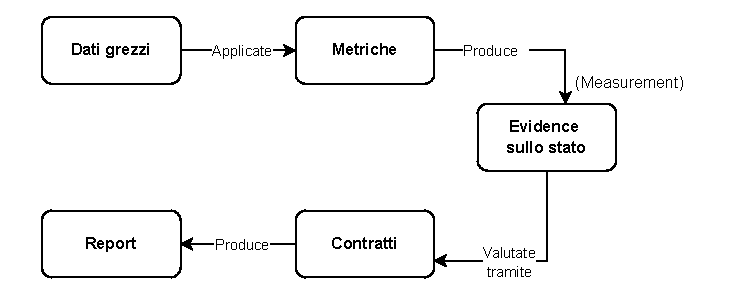
\includegraphics[width=\textwidth,height=0.9\textheight,keepaspectratio]{assets/backup_figures/04_metriche-contratti.drawio.pdf}
\end{frame}

\begin{frame}{Diagramma AE deployato su 3 nodi}
  %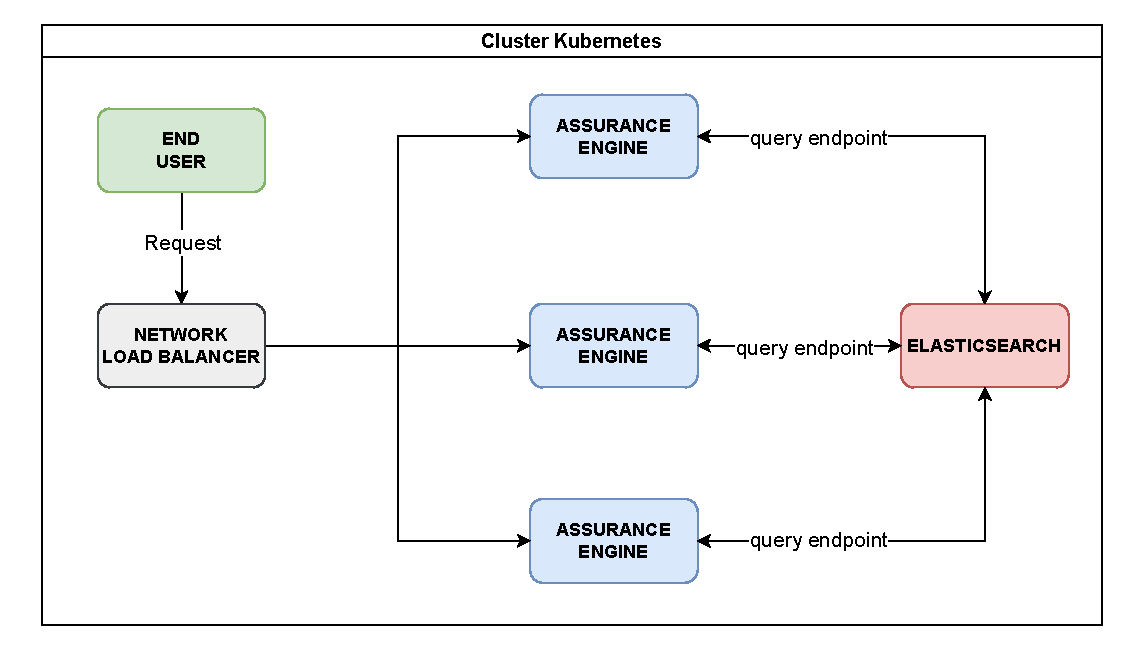
\includegraphics[scale=.55]{assets/backup_figures/05_AssuranceEngine.drawio.pdf}
  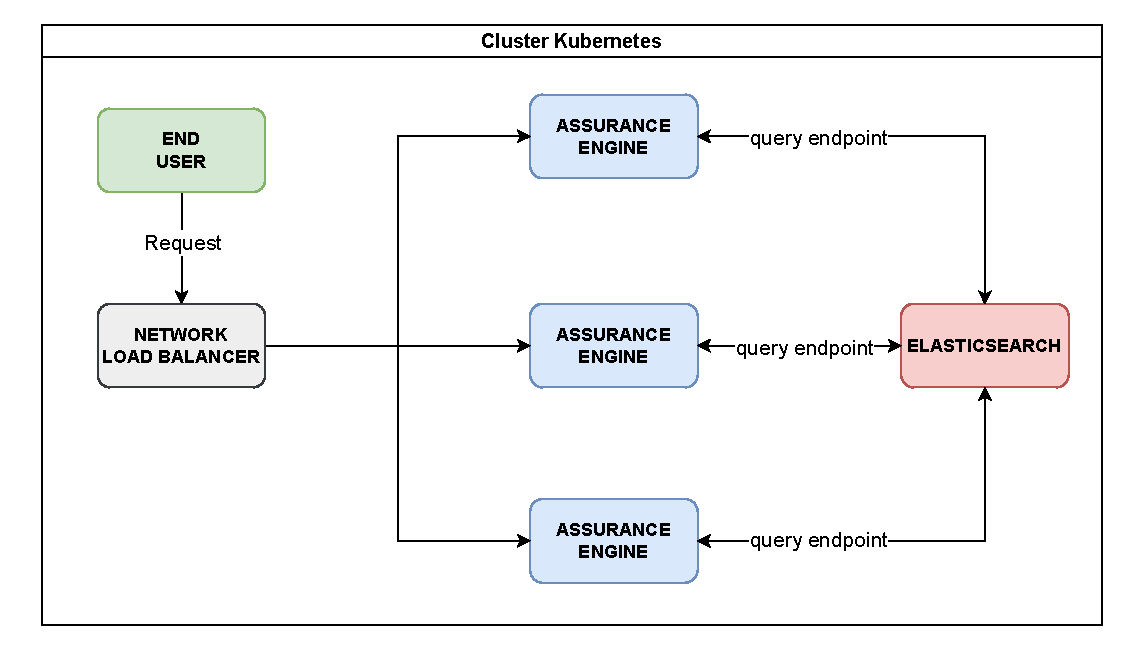
\includegraphics[width=\textwidth,height=0.98\textheight,keepaspectratio]{assets/backup_figures/05_AssuranceEngine.drawio.pdf}
\end{frame}

\begin{frame}{AE flusso di esecuzione}
  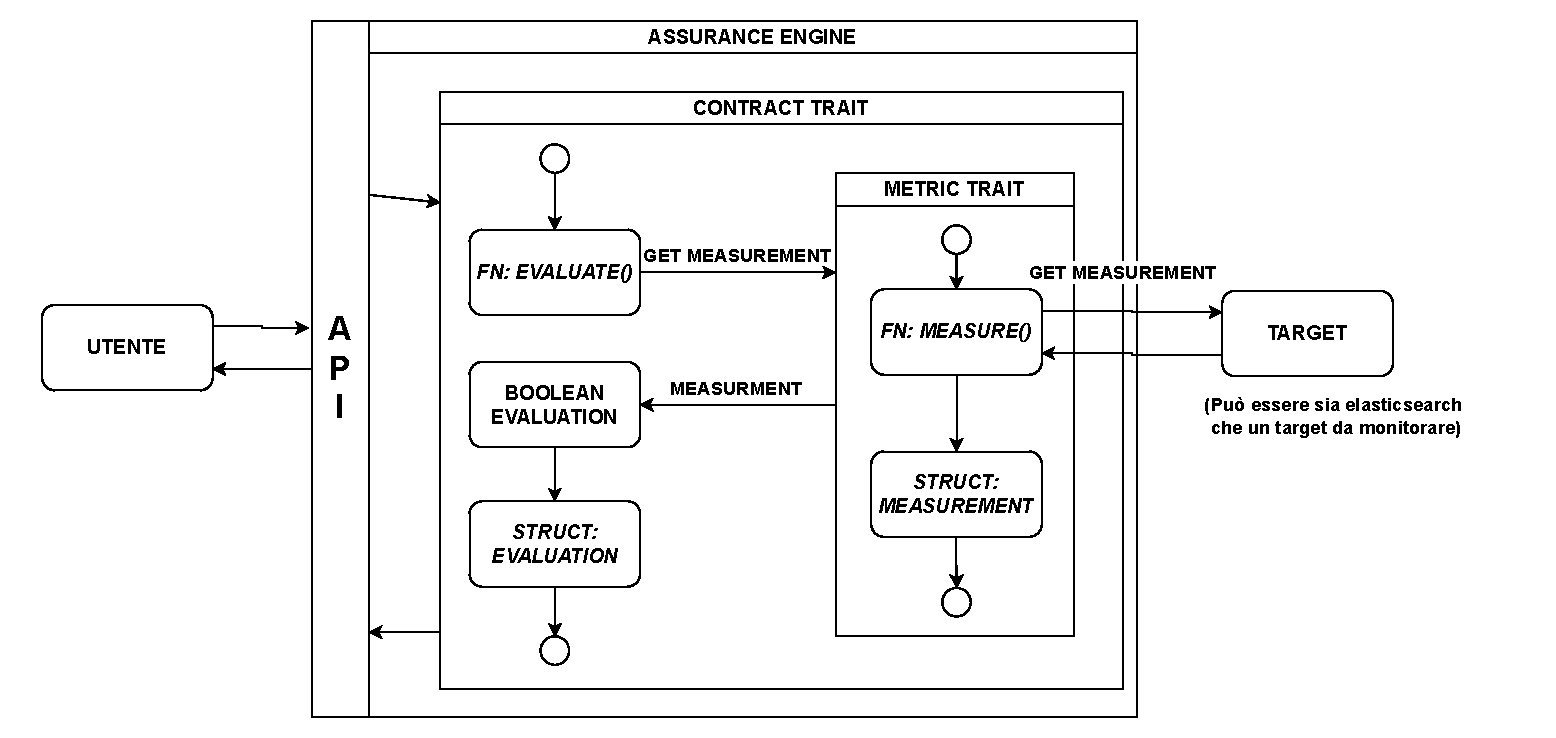
\includegraphics[width=\textwidth,height=0.98\textheight,keepaspectratio]{assets/backup_figures/06_Assurance_engine_flow.drawio.pdf}
\end{frame}

\begin{frame}{Swagger richieste POST}
  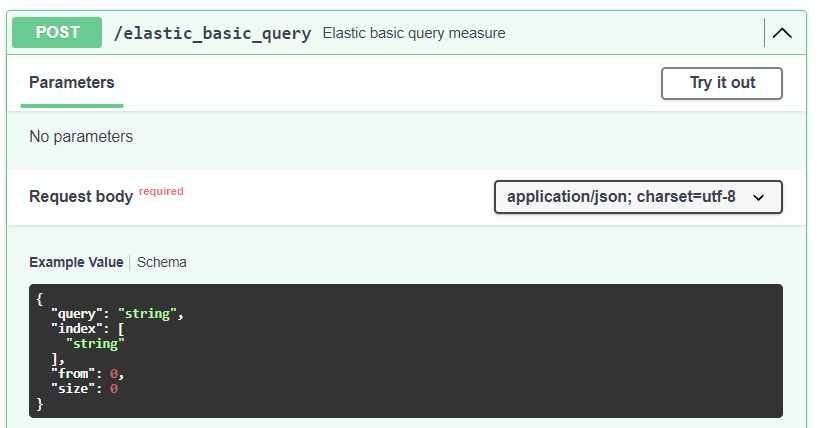
\includegraphics[width=\textwidth,height=0.95\textheight,keepaspectratio]{assets/backup_figures/07_swagger_UI_post.png}
\end{frame}

\begin{frame}{Swagger schema JSON richieste POST}
  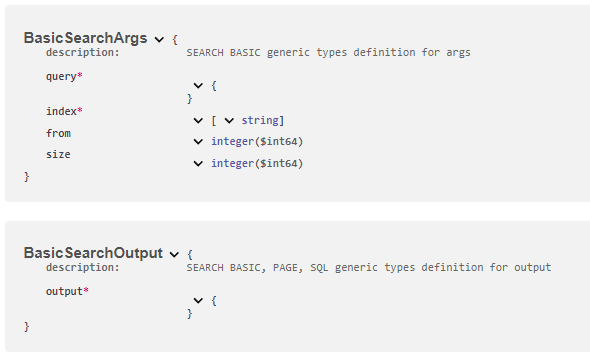
\includegraphics[width=\textwidth,height=0.95\textheight,keepaspectratio]{assets/backup_figures/08_swagger_UI_schema.png}
\end{frame}

\begin{frame}{Diagramma densità probabilistica richieste \texttt{measure} di tipo SEARCH}
  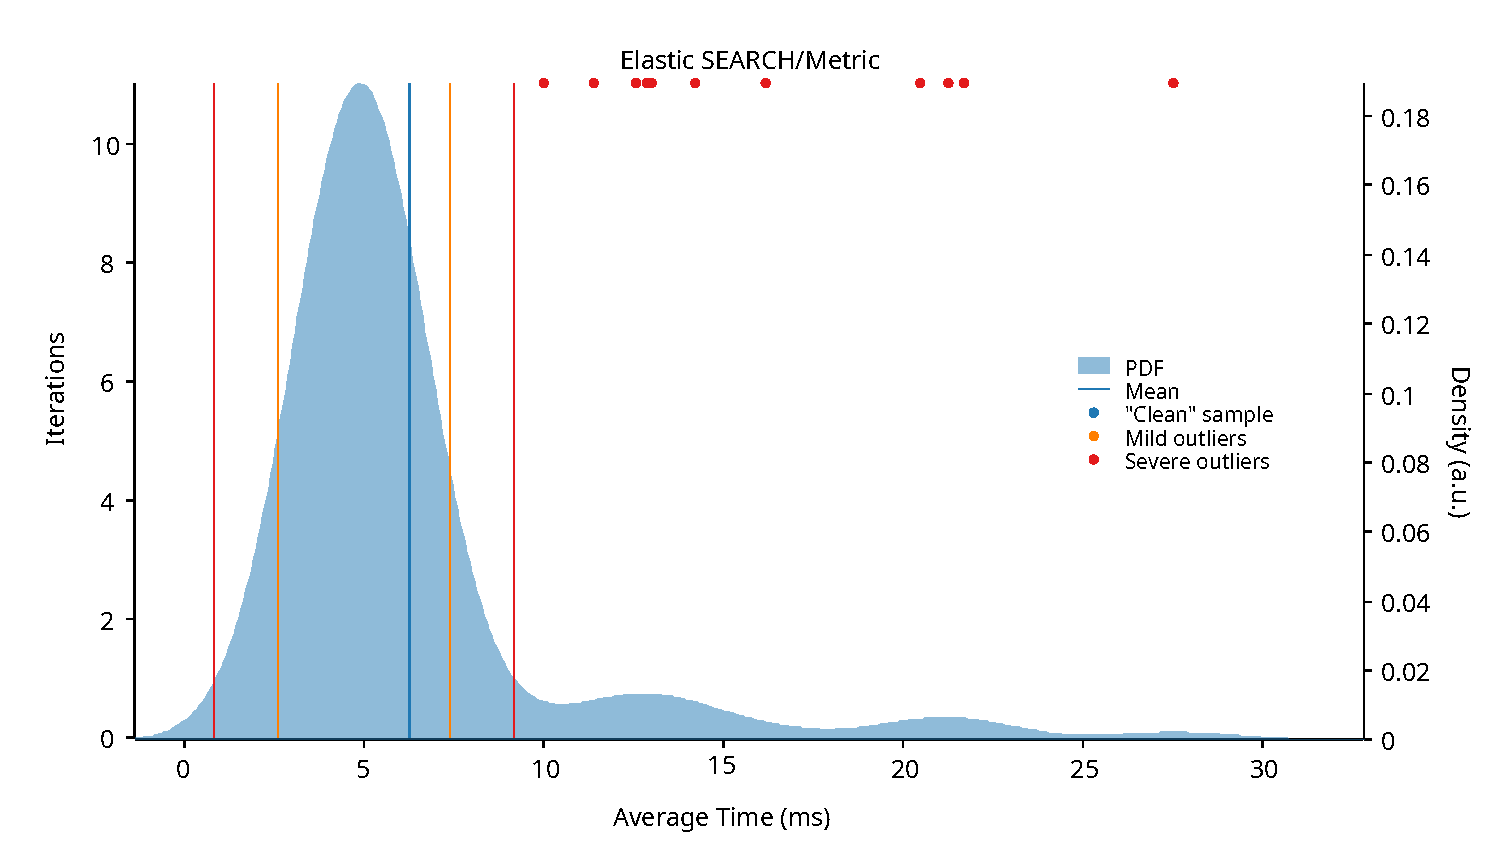
\includegraphics[width=\textwidth,height=0.95\textheight,keepaspectratio]{assets/backup_figures/09_benchmark/SEARCH_metric_density.pdf}
\end{frame}

\begin{frame}{Diagramma densità probabilistica richieste \texttt{evaluate} di tipo SEARCH}
  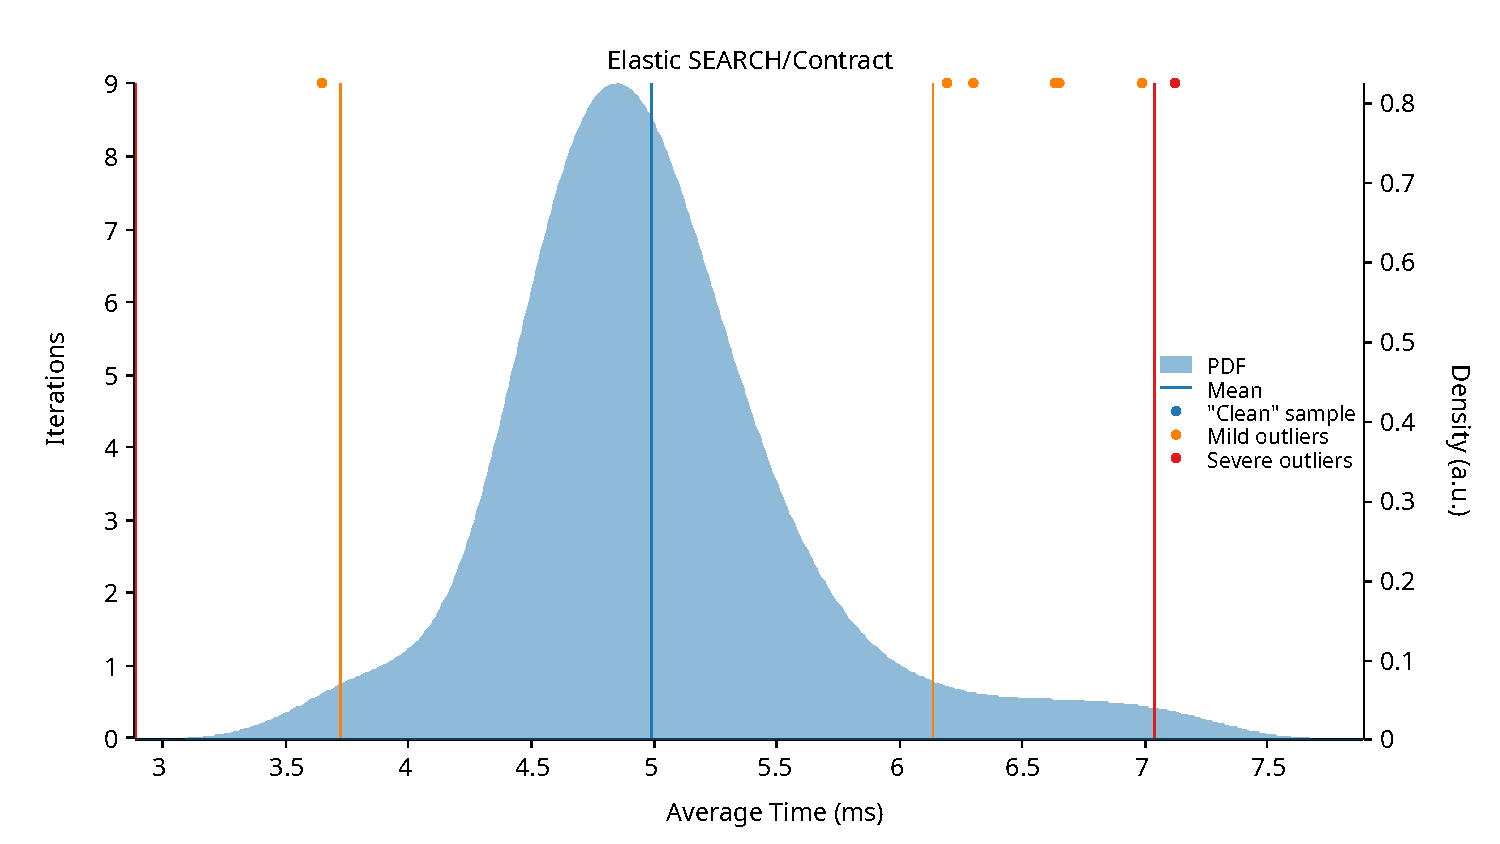
\includegraphics[width=\textwidth,height=0.95\textheight,keepaspectratio]{assets/backup_figures/09_benchmark/SEARCH_contract_density.pdf}
\end{frame}

\begin{frame}{Diagramma densità probabilistica richieste \texttt{measure} di tipo SQL}
  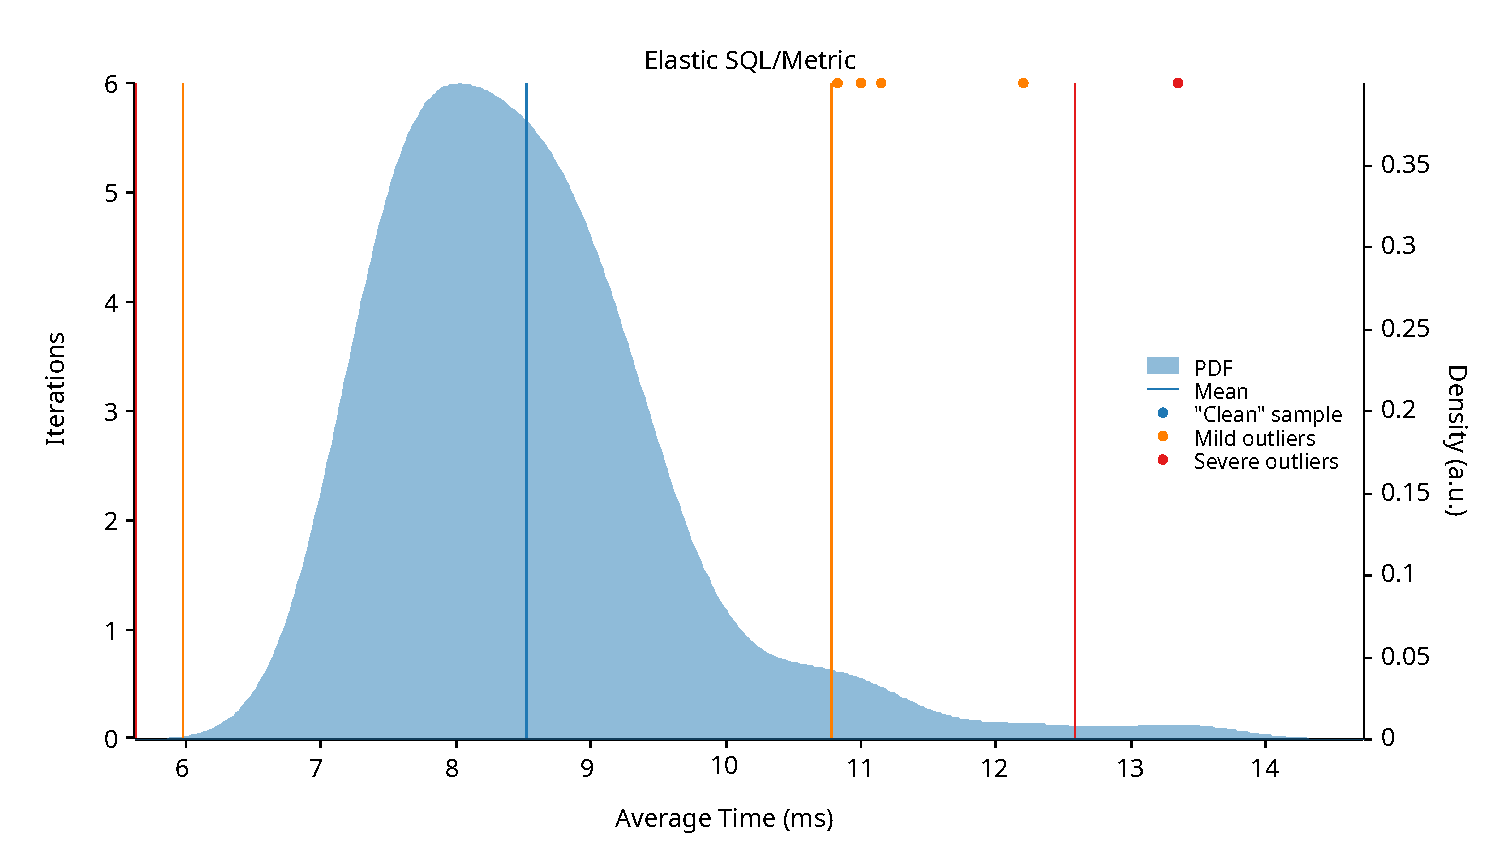
\includegraphics[width=\textwidth,height=0.95\textheight,keepaspectratio]{assets/backup_figures/09_benchmark/SQL_metric_density.pdf}
\end{frame}

\begin{frame}{Diagramma densità probabilistica richieste \texttt{evaluate} di tipo SQL}
  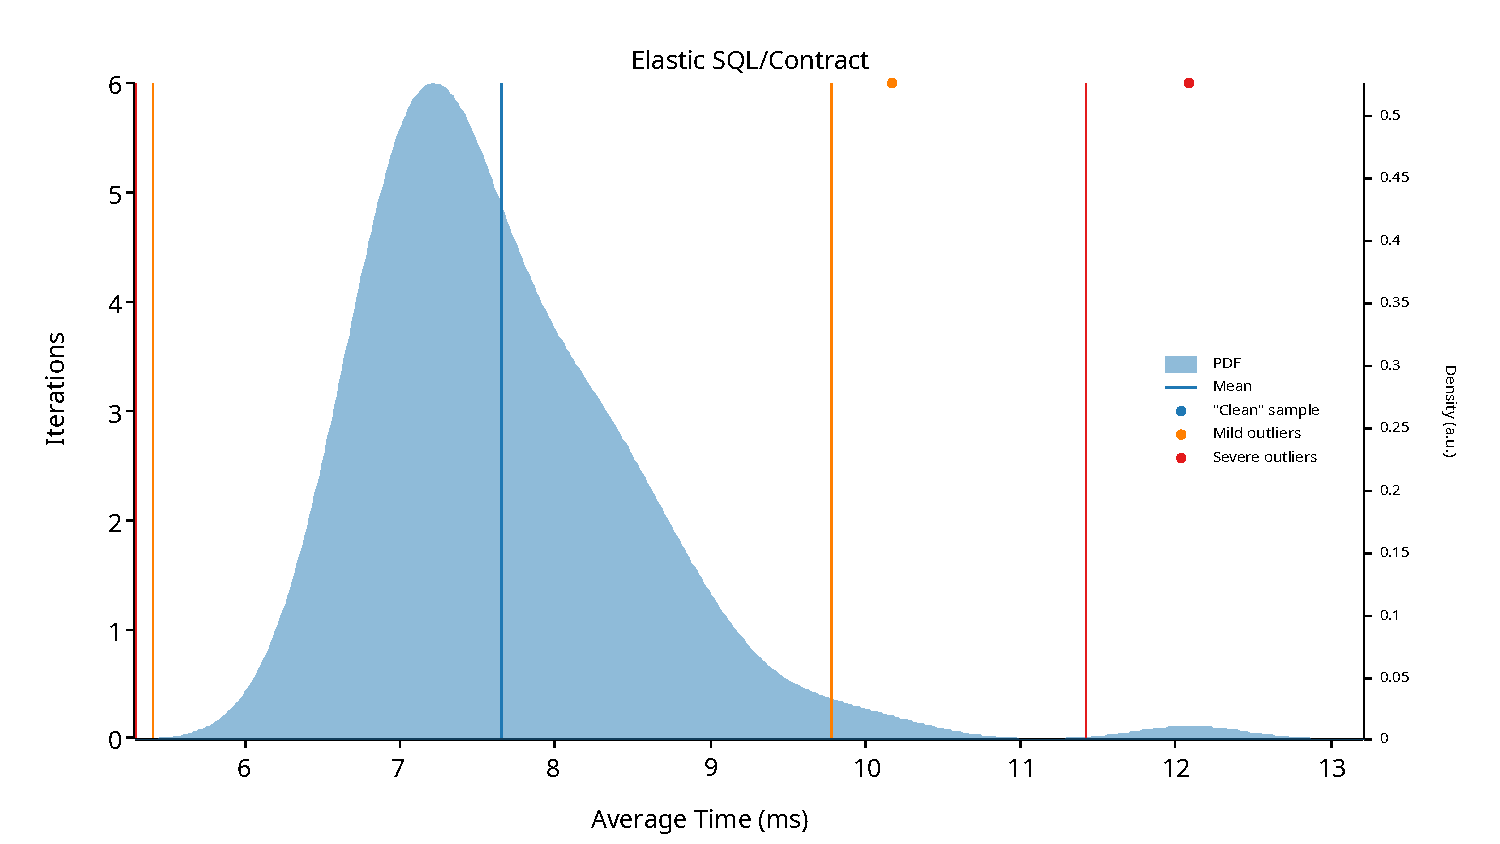
\includegraphics[width=\textwidth,height=0.95\textheight,keepaspectratio]{assets/backup_figures/09_benchmark/SQL_contract_density.pdf}
\end{frame}

\end{document}


